\chapter{OPENSTREETMAP Project}
\begin{figure}[ht]
\centering 
\includegraphics[scale=1]{/home/amisha/gitt/6-weeks-report/input/images/index.jpeg}
\caption{OPENSTREETMAP logo}
\end{figure}
\section{OPENSTREETMAP}
It is a collaborative project to create a free editable map of the world.
Now ,before beginning to make your own tile server, let me explain you some termonologies.
\subsection{Benifit of Having your own tile server}
Maybe you need to have access to you map even when your internet provider is down or when the power is off or both. It won't take much for you to see the benefit of having your own piece of OpenStreetMap infrastructure.\\
Now it's turn to install, setup and configure all the necessary software to operate your own tile server. All the instructions are explained in my blog "https://amisha2016.wordpress.com"\\
These instructions build what OpenStreetMap calls a "tile server". That is, a computer that uses the OSM data set to create map images that are suitable for a web site. Not every OpenStreetMap function is supported, but you will be able to create a local map, keep it up to date and customize it for your own purposes.
\begin{figure}[!ht]
\centering

\includegraphics[width=0.3\textwidth]{input/images/index.png}                   
\caption{Postgresql}
\hspace{-1.5em}
\end{figure}


\subsection{Postgresql / postgis}
PostGIS is a spatial database extender for PostgreSQL object-relational database. It adds support for geographic objects allowing location queries to be run in SQL.\\
Most spatial databases allow representing simple geometric objects such as points, lines and polygons. Some spatial databases handle more complex structures such as 3D objects, topological coverages, linear networks, and TINs.\\
On Ubuntu there are pre-packaged versions of both postgis and postgresql, so these can simply be installed via the Ubuntu package manager.\\
\subsection{Osm2pgsql}
 osm2pgsql is under active development and is best compiled from source.\\
osm2pgsql is a command-line based program that converts OpenStreetMap data to postGIS-enabled PostgreSQL databases.\\
Mapnik is an open source mapping toolkit for desktop- and server-based map rendering, written in C++.\\
One of its many users is the OpenStreetMap project (OSM), which uses it in combination with an Apache Web Server module (mod\_tile) to render tiles that make up the OSM ‘Slippy Map’ Layer.\\
\begin{figure}[!ht]
\centering
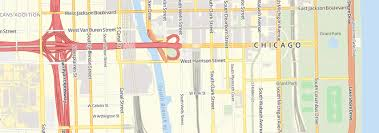
\includegraphics[width=0.3\textwidth]{input/images/bright.jpeg}                   
\caption{Osmbright}
\hspace{-1.5em}
\end{figure}



\subsection{OSMBRIGHT}
OSM Bright is a sensible starting point for quickly making beautiful maps based on an OpenStreetMap database. It is written in the Carto styling language and can be opened as a project in TileMill.\\
The style is still a work in progress and you are encouraged to use the issue tracker to note missing features or problems with the current implementation.\\
\subsection{OpenLayer.js}
OpenLayers makes it easy to put a dynamic map in any web page. It can display map tiles, vector data and markers loaded from any source. OpenLayers has been developed to further the use of geographic information of all kinds. It is completely free.\\
\subsection{Geographic Information Systems (GIS)}
GIS is a computer system for capturing, storing, checking, and displaying data related to positions on Earth’s surface. GIS can show many different kinds of data on one map. This enables people to more easily see, analyze, and understand patterns and relationships\\
The Global Positioning System (GPS) is a space-based navigation system that provides location and time information in all weather conditions, anywhere on or near the Earth where there is an unobstructed line of sight to four or more GPS satellites.\\
\subsection{Change Colors of OSM Map}
For this change your "palette.mss" file.\\
Changes I have made are:-\\
Just change the color of buildings(to red), primary\_line(to green), secondary\_line(to green), road\_halo(to black),standard\_fill(to black).\\
\begin{description}
\item [\$ carto project.mml > OSMBright.xml]


Compiles the file and will do corresponding changes in the file OSMBright.xml\\
\item [\$ sudo -u username renderd -f -c /usr/local/etc/renderd.conf]



\item [\$ sudo /etc/init.d/renderd restart]


The above two commands will re-render


\end{description}


